\chapter{Problem description}
\label{chp:problem-description}

The official long-term goal of the Tribler project is to create a \enquote{create a censorship-free Internet} \cite{pouwelse2012moving}.
The method of the Tribler project is to create a Youtube style service with full decentralisation and robustness against various attacks.
All these features are implemented in a completely distributed manner, not relying on any centralized component.

Numerous initiatives exist around these goals of re-decentralisation, censorship-resilience, and attack-resilient.
However, none of them gathered any significant usage compared to the social media usage levels. 
For instance, Youtube features one billion unique monthly users and there are 1.65 billion monthly active Facebook users.

The problem is that the performance, usability, and features offered by decentralised alternatives are inferior when compared to the experience offered by central solutions.
Creating academically pure self-organising systems such as Tribler has proven to be notoriously difficult.
For example, the extensive list of 194 projects which all aim to create an alternative Internet experience using decentralisations shows the amount of years spent and lines of code produced \cite{redecentralize2016alternative}.
Most of these project are abandoned and few of them have actual real-world usage.

\section{Performance of disk I/O}
The Tribler project created a roadmap to offer the same service, features, user experience, and performance as the YouTube video-on-demand service.
Tribler has no dependency on central service infrastructure, does not need profit or advertisements to generate revenue, and even can function without Internet connectivity. However, especially the poor performance of Tribler is hampering wide-spread usage. Figure~\ref{fig:tribler_roadmap} shows part of the six main uncompleted roadmap items.

\begin{figure}[h]
	\makebox[\textwidth][c]{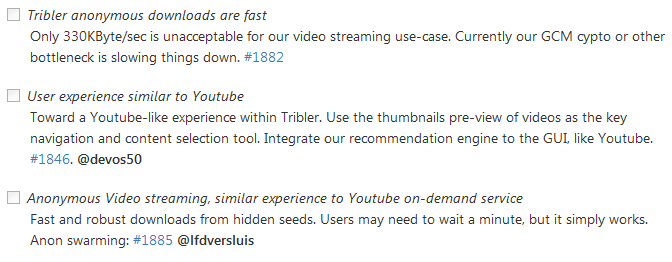
\includegraphics[width=\linewidth]{problemDescription/images/roadmap}}
	\caption{Three of the six uncompleted roadmap items.}
	\label{fig:tribler_roadmap}
\end{figure}

The problem we address within this thesis is the underlying reason for poor performance and unacceptable user performance. Measurements dating back from 2014 indicate that Tribler performance is IO-bound.
Especially with slow hard disks, but also with fast SSD storage the main performance bottleneck seems to be around database access.
With our focus on the fundamental issue we believe we can make a significant step forward in making decentralized technology ready for large-scale usage. 

\section{Tribler database dependency}

All information within Tribler is stored in a database for persistence and ease of use.

Insert picture Dispersy SQL:
[https://camo.githubusercontent.com/eae1fe5cce8095a934d48aa7b80cd752c672800f/68747470733a2f2f662e636c6f75642e6769746875622e636f6d2f6173736574732f313734313633322f3239303637352f32303935393466632d393265632d313165322d386264332d3463626434303335323964302e706e67]

This database is becoming a key performance bottleneck.
Insert picture MBytes/hour : [https://github.com/Tribler/tribler/issues/564]

\section{asynchronous IO}

The challenge we address in this thesis is attempting to remove this performance constraint by replacing all blocking IO calls with asynchronous non-blocking IO. 

Example:
Instert picture like: [https://userscontent2.emaze.com/images/67f41361-9c9a-45c3-9a81-a4c49d5a66c8/95ba8eb4-aa59-4dab-992e-adcb38cf9d8c.jpg]

\section{Improved developer productivity}
Refactoring.. important.. continous changes.. expand features...
By using a database manager to handle asynchronous IO we also improve developers productivity, another vital performance measure. Less code and improved readability enhances productivity...



\section{OLD TEXT}
Only by comparing different builds can one gain insight into performance changes.
Currently Tribler lacks this insight.
As Tribler is heavy IO-based and likely IO-bound, it is crucial to have these numbers.
A breakdown of database statements is needed and the amount of IO that is generated.
Recently a block-chain like structure called the Multi-Chain was added to Tribler and soon another feature called credit mining will be introduced as well.
The impact and increase of IO caused by these additions are unknown.

Ideally, we would like to run regression tests on multiple platforms powered by our Jenkins continuous integration system as visualized by Figure X \todo{make figure.}.
This regression test will feature average use cases and automatic graph generation to give developers an instant overview of their changes.
This system has to run automatically whenever a pull request is opened on GitHub.
Efforts can then be made to optimize the IO output and improve the performance of Tribler.

\section{Resolving bottlenecks}
To improve the performance of Tribler, (IO) bottlenecks to need to be removed.
The key problem here is how to identify and resolve bottlenecks in a complex system such as Tribler.

By careful inspection of the usage of IO, we identified that Tribler's IO is blocking the main thread.
Many programming languages have support for parallelization, allowing multiple functions to be executed at the same time by using threads.
Tribler does not have access to this paradigm as it's written in the Python programming language.
Python lacks this feature as only one thread can run in the Python interpreter at any time because of the Global Interpreter Lock (GIL).
However, a thread does release the GIL when it's performing a blocking IO operation, allowing other threads to get a hold of the GIL and run.
Leveraging this trait to gain performance is a huge step forward towards solving the (IO) bottleneck Tribler is currently facing.

\section{Tribler's code base}
At the same time, Tribler's current code base has a severe lack of (unit) tests, structure and documentation and contains dead code.
The current version has been in development for over nine months, is plagued with bugs and non-functioning on some platforms.
As of writing, the code is only tested on a single Unix operating system.
Tribler, however, is available for all three major operating systems: Windows, Mac OS and Unix distributions.
As users are reporting platform specific bugs, it is evidently important that automated testing on all three platforms are realized.
All this results in long and complex debugging processes and creates a steep learning curve for new students joining the project and might withhold members of the open-source community to start contributing.

While it's not this thesis primary goal, refactoring the code involved with the bottlenecks and properly documenting and testing this refactored code is a secondary goal of this thesis, aiding in lowering the learning curve and improving the stability of the Tribler code base.

% \section{Connectability}
% One of the problems Tribler faces is the connectability of its users.
% Users can be behind e.g. firewalls that prevent incoming or outgoing connections.
% Currently, Tribler employs NAT and Firewall Traversal [CITE], yet the success of this method is limited.
%The Tribler team has implemented their own Distributed Hash Table (DHT) in python while existing libraries such as LibTorrent also offer these.
% These implementations should be tested to see if changing to a library offers a significant boost in terms of exchange or speed.

%When users are downloading anonymously, they are inside so-called `hidden swarms'.
%These hidden swarms are not present in e.g. LibTorrent's DHT and therefore information from peers has to be exchanged between peers themselves by means of introducing peers to each other (PEX).
%By making use of Dispersy, Tribler creates rendezvous points to introduce peers to each other.
%If these rendezvous points are not connectible, PEX cannot take place.
%Solving this may be done by always connecting to the same port (chosen by the user or a default) and ask the user to forward that port.
%If users are not willing to do so, they can be penalized.
%This penalty can be for example not able to download anonymously at all, receive half the amount of credits when credit mining (see [CITE]) or limited download speed.

% \section{Anonymous download speed}
% To allow for anonymous downloading, Tribler uses a Tor-like technique to create so called `anon tunnels'.
% To increase download speed and prevent a bottleneck in the network hampering the overall download speed, several tunnels are built to download simultaneously from [CITE?].
% Since this Tor-like technique includes cryptographic functions, having multiple tunnels running concurrently results in a lot of cryptographic calls being executed.
% Stok et al. profiled Tribler using a gumby\footnote{Gumby is Tribler's experiment running framework.} experiment. This experiment showed that a lot of processing time is spent on encrypting and decrypting packets [CITE] as well as serializing and deserializing data.
% Currently, the CPU power is a bottleneck when downloading using the anonymous tunnels.
% By offloading the encryption and decryption of packets to a separate core, the workload on the core on which Tribler is running can be reduced.
% This should yield an increased download speed and better spread of workload overall as more packets can be processed per time unit.

% \section{Package serialization}
% One of the core components of Tribler is Dispersy. 
% Dispersy is a fully decentralized elastic database capable of communicating packets and exchanging peers.
% Both Dispersy and Tribler make use of python' built-in serialization function.
% The profile ran by Stok et al. [CITE] indicated that a significant amount of CPU resources is spent on serializing data when sending or receiving UDP packets.
% As previously explained, running multiple threads at once does not result in code being executed concurrently.
% Cap'n Proto is a serialization framework that offloads the serialization of packets to a C++ process, which bypasses the global interpreter lock.
% This means that the other threads -- who are still affected by the global interpreter lock -- can immediately continue their work as the locks is released once the offloading to the C++ code base is done.

% \section{Responsiveness}
% Since Tribler is written in the python language, calls on any thread will cause other threads to halt their execution. % this is wrong.
% Normally two separate threads can run code in parallel as they generally do not touch each other's state.
% The cause of this is the Global Interpreter Lock (GIL) which states that only one function can be executed at a time.
% In its current state, the Graphical User Interface (GUI) of Tribler will block if it's doing some CPU or IO intensive work.
% This yields a scenario in which the user is unable to perform any action, which is not user friendly.
% In some cases the operating system itself will show e.g. a warning or visualisation that the process is not responding.
% To solve this issue, heavy operations should be done on separate threads or processes which are not monitored by the GIL.
% Several libraries that are written in C/C++ are a good example of this.
% Once the code of such a library is invoked and the execution is offloaded to the C/C++ code, the GIl is released, allowing other python code to ran in parallel.
% Another approach is using the python framework Twisted.
% Twisted has implemented a thread pool that also bypasses this GIL.
% By rewriting CPU or IO intensive code to make use of this thread pool in an asynchronous way, the responsiveness of Tribler can be improved.

% \section{Code quality and testing}
% Tribler's current code base is in a bare state.
% The current version that has been in development for over nine months now is plagued with bugs and is non-functioning.
% Furthermore, there is a severe lack of unit tests, a lot of the code is undocumented and unnecessary complex and structure and flow are missing.
% This results in long and complex debugging processes when bugs are found and raise the bar for new contributors to get familiar with the code base.

% As of writing, the code is only tested on a single Unix operating system.
% Tribler, however, is available for all three major operating systems: Windows, Mac OS and Unix distributions.
% As users are reporting platform specific bugs, it is evidently important that automated testing on all three platforms are realized.

% Refactoring the code is necessary in order to regain the structure and lower the code complexity.
% Furthermore, proper unit tests are required to ensure Tribler's stability now and in the future.
% These tests have to be executed on build machines that run different operating systems, preferably with various configurations e.g. 32 and 64 bit architectures or different library versions.

\section{Objective and research questions}
\label{chp2:sct:objectives-research-questions}
The objective of this thesis is to introduce a IO regression test system and to improve the performance and responsiveness of Tribler.
The verification of the system is done by focussing on removing bottlenecks present.
These improvements will be applied by means of refactoring current code, which is largely undocumented, poorly tested and unnecessary complex.
In general, projects facing similar issues can adopt the practices applied when changes made to the Tribler code base.\\

The research presented in this thesis was carried out in cooperation with the Tribler team. 
The Tribler team consists of both staff members of the Technical University of Delft as well as Bachelor and Master students.
In total Tribler has been in development for over 10 years and the project has received contributions from more than 40 contributors.
Using the knowledge of a senior developer still present, known issues of Tribler could be noted down immediately to which resulted in a set of diverse tasks to complete.
Based on the objectives of Tribler, this thesis aims to answer the main research question formulated below.\\

\textbf{Main Research Question:} How can we improve Tribler's performance, responsiveness and code base by means of refactoring?\\

To answer this main research question, we have defined three research questions below. Each of these research questions will be justified as why they contribute to the main research question.\\

\textbf{Research Question 1:} How can we identify bottlenecks in a complex system such as Tribler?\\

Software projects such as Tribler are often dependent on libraries i.e. third party code and combine several components or modules to form a program.
To improve the performance of such a system, one needs to be able to identify bottlenecks.
Bottlenecks are parts of the code where often performance and responsiveness can be gained. 
Sometimes by implementing a more efficient algorithm or by introducing parallelization these bottlenecks can be resolved.
Identifying these bottlenecks is the first step to resolve them.\\

\textbf{Research Question 2:} Can a system such as Tribler benefit from asynchronous programming?\\

To improve performance and responsiveness, parts of Tribler can be rewritten to become asynchronous.
By performing tasks asynchronously the performance and responsiveness of a program can improve.
However, an asynchronous approach can have its drawbacks. 
One of these drawbacks is that it requires a different mindset for the programmers as the whole call chain and structure of a program becomes different.
Identifying these drawbacks and deciding if the benefits outweigh the costs is necessary to prevent the current state from worsening. \\

\noindent
\textbf{Research Question 3:} How do we incorporate benchmarking and regression testing into Tribler to gain insight into performance statistics?\\

To be able to conclude performance has improved, we need to benchmark current and new code using a regression testing system.
The key issue here is to define metrics and workloads to benchmark with.
If the metrics do not represent a realistic use-case the benchmark may be flawed, rendering the outcome unreliable and inaccurate.

Additionally, the regression testing system should not clog the throughput of the current test architecture.
Running a one hour benchmark per change per pull request will hog the system and will severely strain the development speed.

\section{Main contributions}
The main contribution this thesis offers are as follows.
We introduce a regression testing system that benchmarks different versions of the same code base to gain insight into performance metrics such as disk IO.
Next, to present the working of said system, we present methods to identify bottlenecks in a complex system such as Tribler. 
We elaborate on the subject of multitasking and parallelization in the context of the Python programming language and provide arguments where asynchronous programming is preferred over synchronous programming, using Tribler as a case study.
Finally, experimental results and measurements will be provided to confirm the main goal of this thesis i.e. improving responsiveness, code quality and performance.
